\section{Results}\label{sec:results}
In this section, the impact assessment for all of the considered test cases from the previous section are developed. With this in mind, two assessments are conducted for each test case. 

Initially, a midpoint assessment is conducted to compare the impact of each note-taking scenario across various environmental mechanisms. This assessment is carried out both comparatively and in absolute terms, aiming to not only highlight the differences in impact between the approaches but also provide context regarding the significance of each category. For instance, while the digital scenario may exhibit a five-times greater impact in a specific category compared to the analog case, if the absolute value remains relatively small, it limits the extent of conclusions that can be drawn from this relationship. In this evaluation, all absolute values are expressed in units such as loss of species per year (species.yr), disability-adjusted life years (DALY), or excess costs in 2013 US Dollars. These units represent the damage to the ecosystem quality, damage to human health, and cost increases due to resource scarcity caused by the note-taking approach, respectively.

Following the midpoint assessment, an endpoint assessment is conducted to establish a single-score comparison between the approaches using normalization factors. This comparison step has a higher level of uncertainty compared to the previous assessment since it requires qualitative input to determine normalization factors across all categories. However, the well-established ReCiPe methodology used in this study provides objectivity to these values to the best of our knowledge.

% Include subsection showing the inventory for both cases maybe

\subsection{Manufacturing Impact}\label{subsec:results_manufacturing}
As mentioned in the previous section, first, the manufacturing processes for both note-taking approaches are compared. For this, the previously mentioned scenarios including their transportation and waste treatments are considered. 

As a first step, their effects per impact category were compared. Figure~\ref{fig:characterization_manufacturing} depicts a relative analysis for the most significant categories between both scenarios while Figure~\ref{fig:characterization_table_manufacturing} shows the absolute values for all impact categories.


\begin{figure}[H]
    \centering
    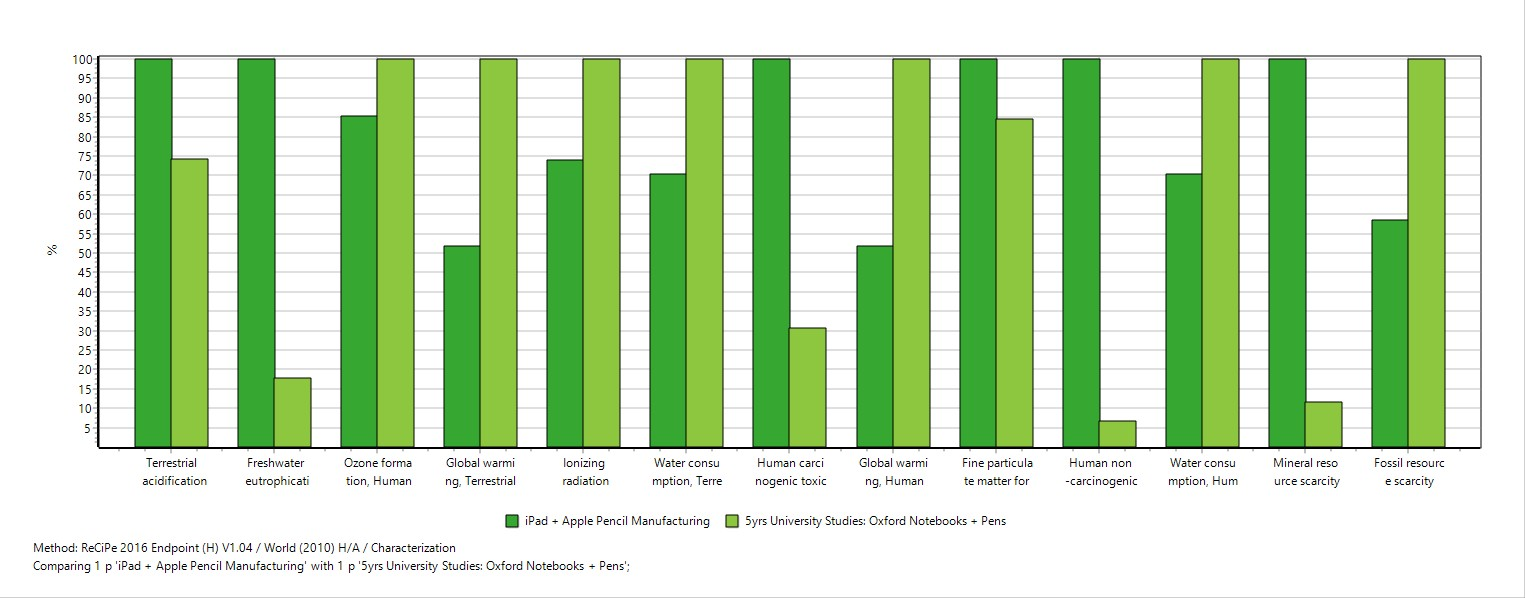
\includegraphics[width=\textwidth]{images/Manufacturing/Characterization_Manufacturing.JPG}
    \caption{Relative midpoint assessment for the manufacturing of the investigated note-taking approaches per impact category.}\label{fig:characterization_manufacturing}
\end{figure}

This Figure showcases the similarity between the impact for both note-taking scenarios where each case dominates six categories. However, a clear disparity favoring the digital approach can be seen for all categories related with global warming and natural resources. The analog case causes about twice as much global warming on average over the three considered categories and is well above the digital case for scarcity of fossil resources, water consumption and ozone formation. On the other hand, the digital case has a much greater impact in categories involving the damaging of ecosystems such as terrestrial acidification and freshwater eutrophication as well as human impacts (carcinogenic and non-carcinogenic) and scarcity of mineral resources.

\begin{figure}[H]
    \centering
    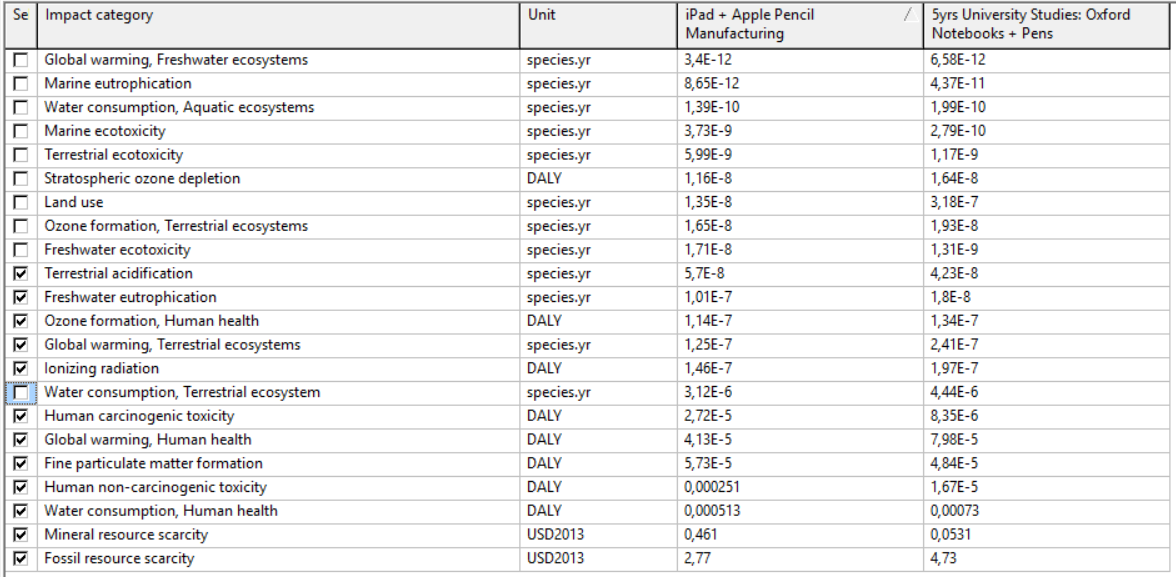
\includegraphics[width=0.9\textwidth]{images/Manufacturing/Characterization_Table_Manufacturing.PNG}
    \caption{Absolute midpoint assessment for the manufacturing of the investigated note-taking approaches per impact category.}\label{fig:characterization_table_manufacturing}
\end{figure}

From Figure~\ref{fig:characterization_table_manufacturing}, the same trend is observed. Terrestrial ecotoxicity caused by the digital case is more than five times larger than for the analog case, whereas the land use for the analog case is an entire order of magnitude larger than the digital case. Nevertheless, these remaining categories are orders of magnitude smaller than the ones described in the previous Figure and must be carefully analyzed as to not allow for the attention to be deviated from the impact categories with the majority of the impact share. 

Once the midpoint assessment is conducted, the impact categories can be divided into three main groups based on the recipient for their impacts: the ecosystem, human health and the global resources. Figure~\ref{fig:damage_assessment_manufacturing} showcases a relative comparison per category between both note-taking scenarios.

\begin{figure}[H]
    \centering
    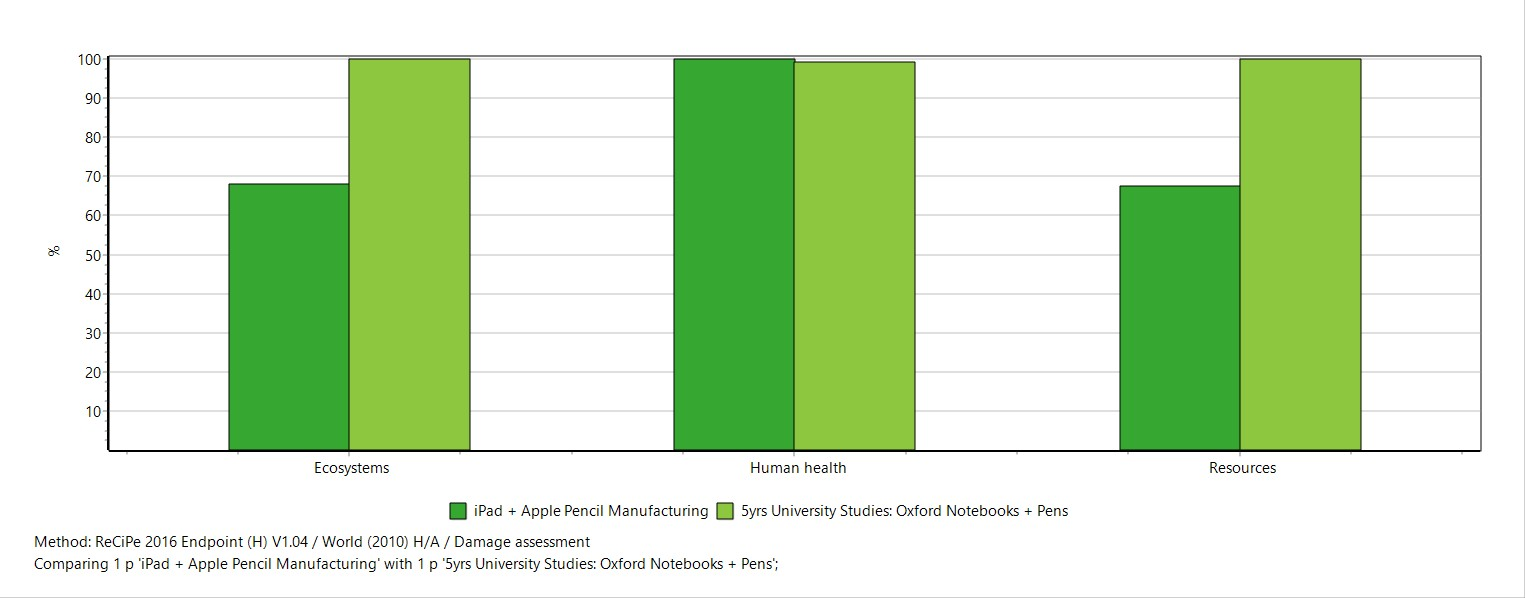
\includegraphics[width=\textwidth]{images/Manufacturing/Damage_Assessment_Manufacturing.JPG}
    \caption{Relative endpoint assessment for the manufacturing of the investigated note-taking approaches.}\label{fig:damage_assessment_manufacturing}
\end{figure}

Based on these findings, it is apparent that both manufacturing processes exhibit a comparable impact on human health, with a slight advantage observed for the digital scenario. However, the analog scenario demonstrates approximately a 40\% greater impact on the ecosystem and global resources. This discovery is particularly unexpected, considering the significant manufacturing requirements and intercontinental transportation involved in the digital scenario.

Nevertheless, similar to the midpoint assessment, analyzing the absolute scores for each category is imperative for the context of this difference. Figure~\ref{fig:single_score_manufacturing} depicts the total single score given to the manufacturing for both note-taking scenarios alongside their internal distributions. 

\begin{figure}[H]
    \centering
    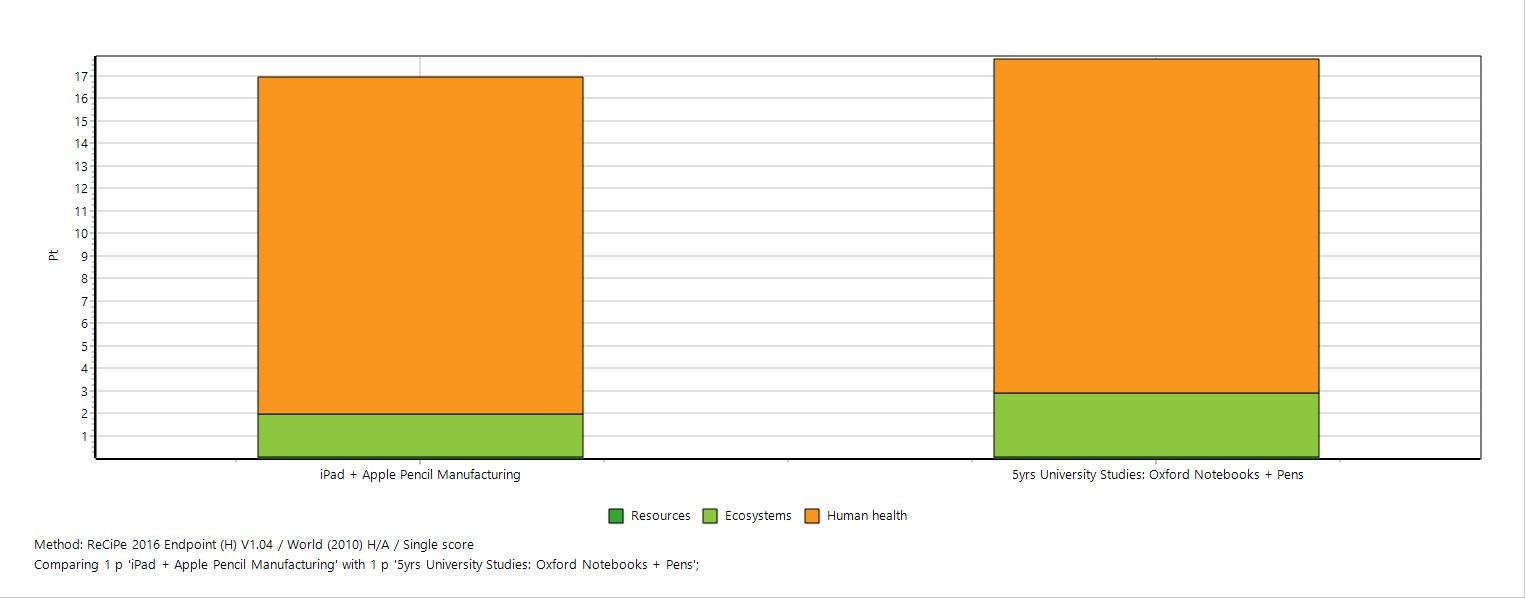
\includegraphics[width=\textwidth]{images/Manufacturing/Single_Score_Manufacturing.JPG}
    \caption{Single score distribution for the manufacturing of the investigated note-taking approaches.}\label{fig:single_score_manufacturing}
\end{figure}

From here, it becomes evident that the impact on human health is the major contributor for both scenarios, with the 40\% increase in ecosystem and resource impact for the analog scenario amounting to a surplus of an individual single score point. 

\subsection{Life Cycle Impact}\label{subsec:results_life_cycle}
Once the manufacturing for both note-taking scenarios was compared, the energy required to power the electronics from the digital case are taken into account. As mentioned earlier, three energy source scenarios are considered ranging from 0 to 100\% RES penetration for the grid mix. The results for their midpoint and endpoint assessment comparisons are seen in the following.

\subsubsection{0\% RES Penetration}
As expected, the impact for the digital case increases massively when the energy required to charge and operate the electronics is considered. Figures~\ref{fig:characterization_RES_0} and~\ref{fig:characterization_table_RES_0} showcase the midpoint assessment for both scenarios with 0\% RES penetration.

\begin{figure}[H]
    \centering
    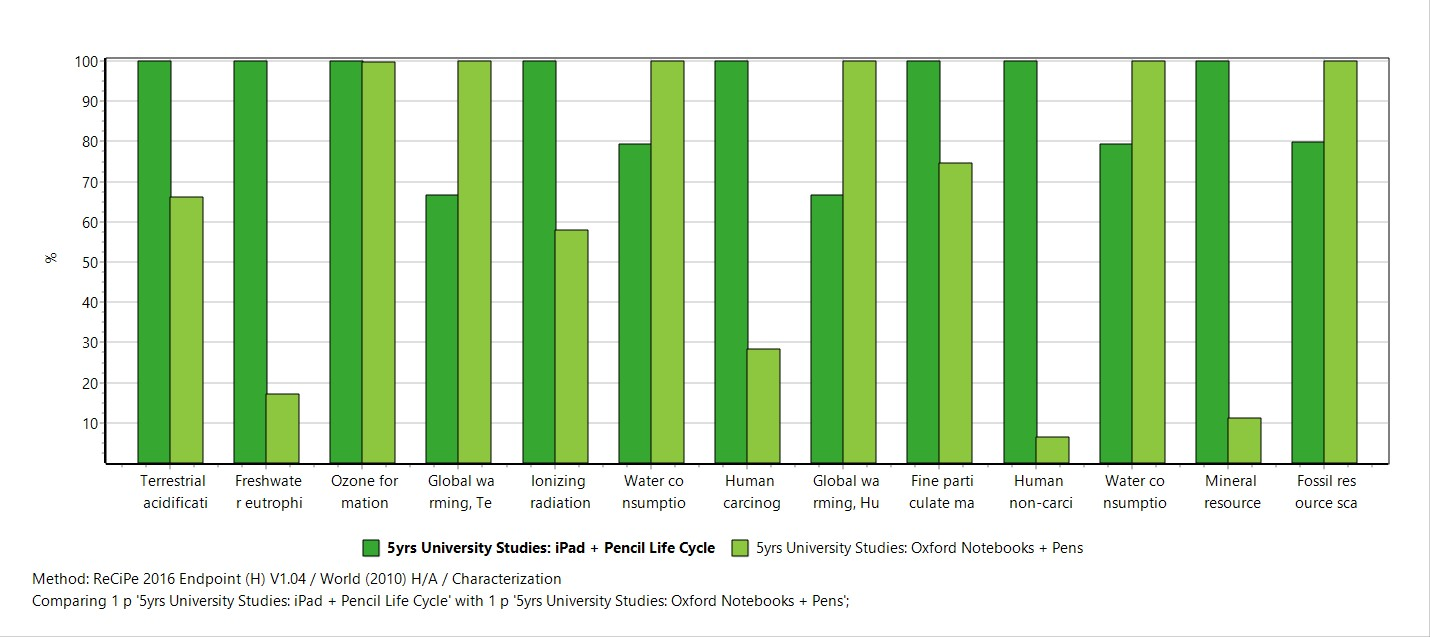
\includegraphics[width=\textwidth]{images/RES_0/Characterization_RES_0.JPG}
    \caption{Relative characterization for a 0\% RES penetration scenario of the investigated note-taking approaches per impact category.}\label{fig:characterization_RES_0}
\end{figure}

From Figure~\ref{fig:characterization_RES_0} it becomes evident that the impact caused by the energy required to run the electronics causes for the digital case to far outweigh the impact for the analog case. The analog case represents no more than 20\% of the impact caused by the digital case across all categories, with most being below 15\%.

\begin{figure}[H]
    \centering
    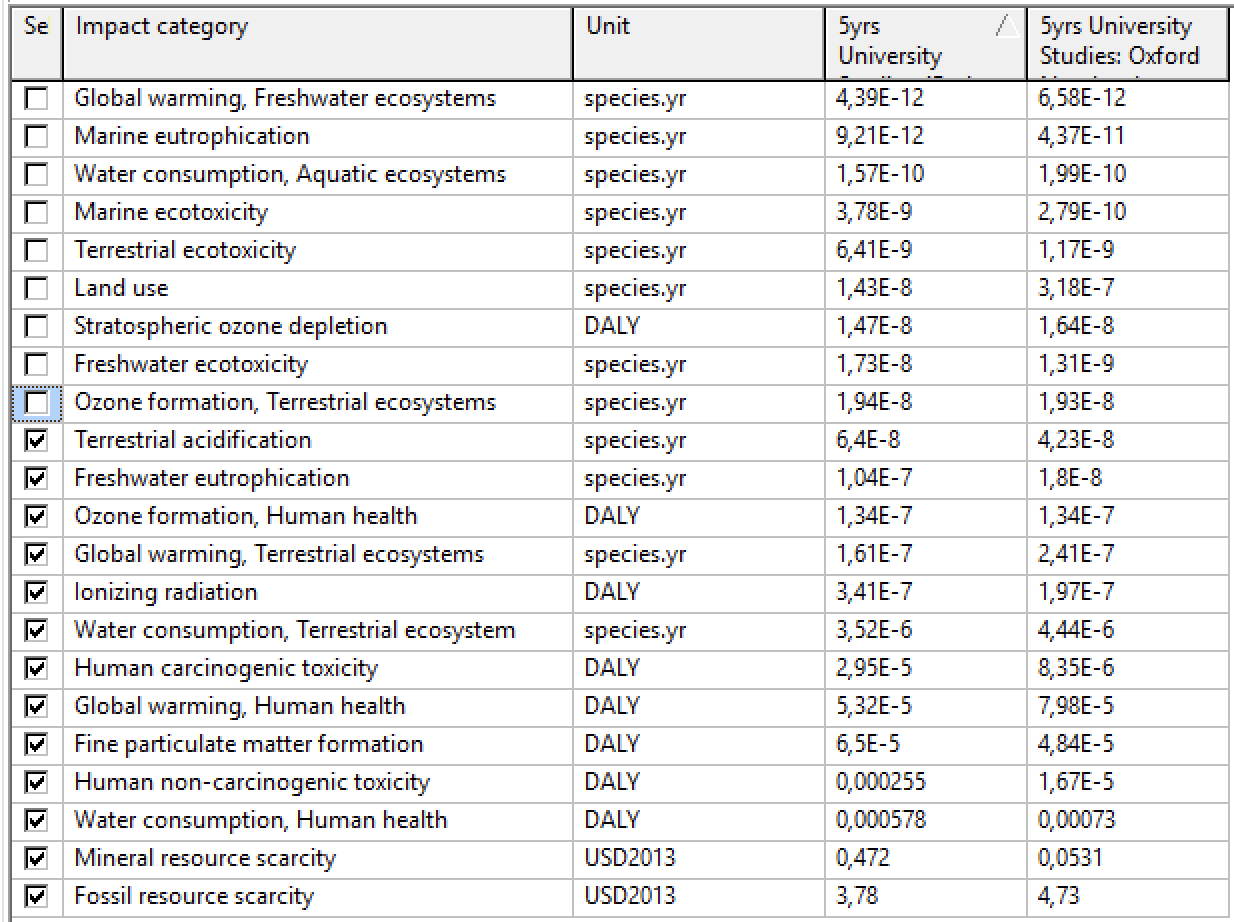
\includegraphics[width=0.9\textwidth]{images/RES_0/Characterization_Table_RES_0.PNG}
    \caption{Absolute characterization for a 0\% RES penetration scenario of the investigated note-taking approaches per impact category.}\label{fig:characterization_table_RES_0}
\end{figure}

\begin{figure}[H]
    \centering
    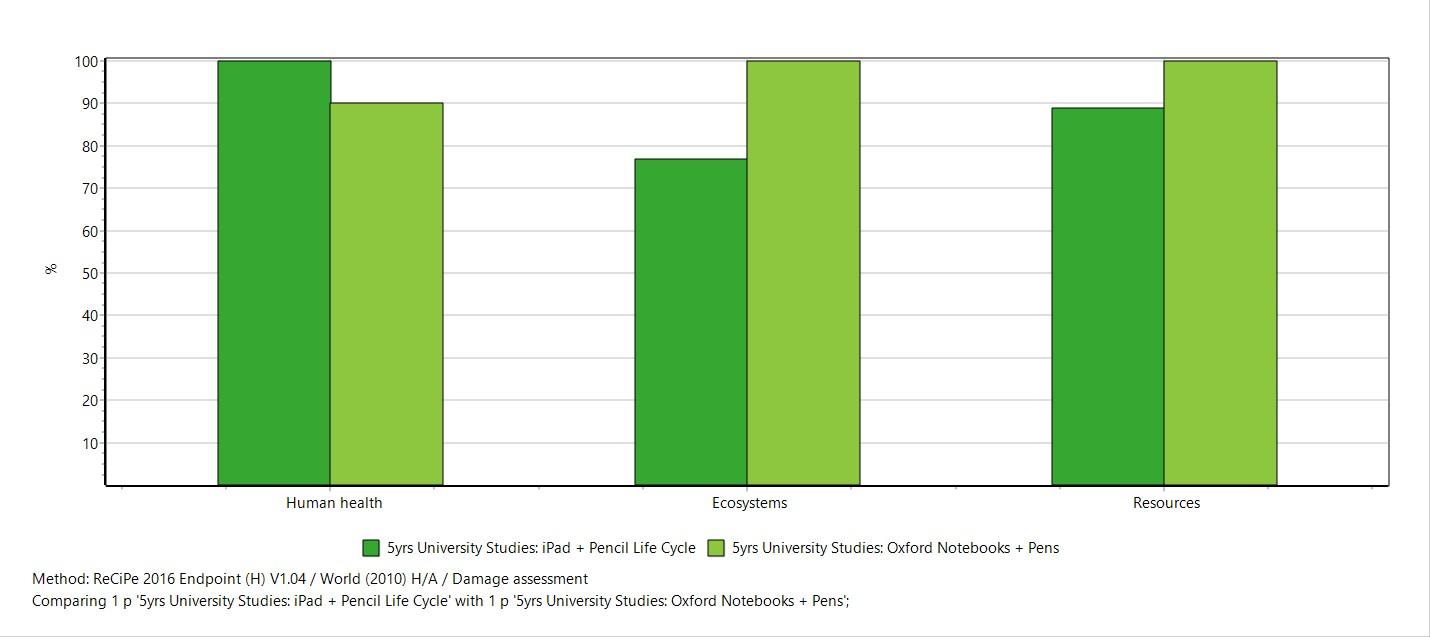
\includegraphics[width=\textwidth]{images/RES_0/Damage_Assessment_RES_0.JPG}
    \caption{caption}\label{fig:damage_assessment_RES_0}
\end{figure}

\begin{figure}[H]
    \centering
    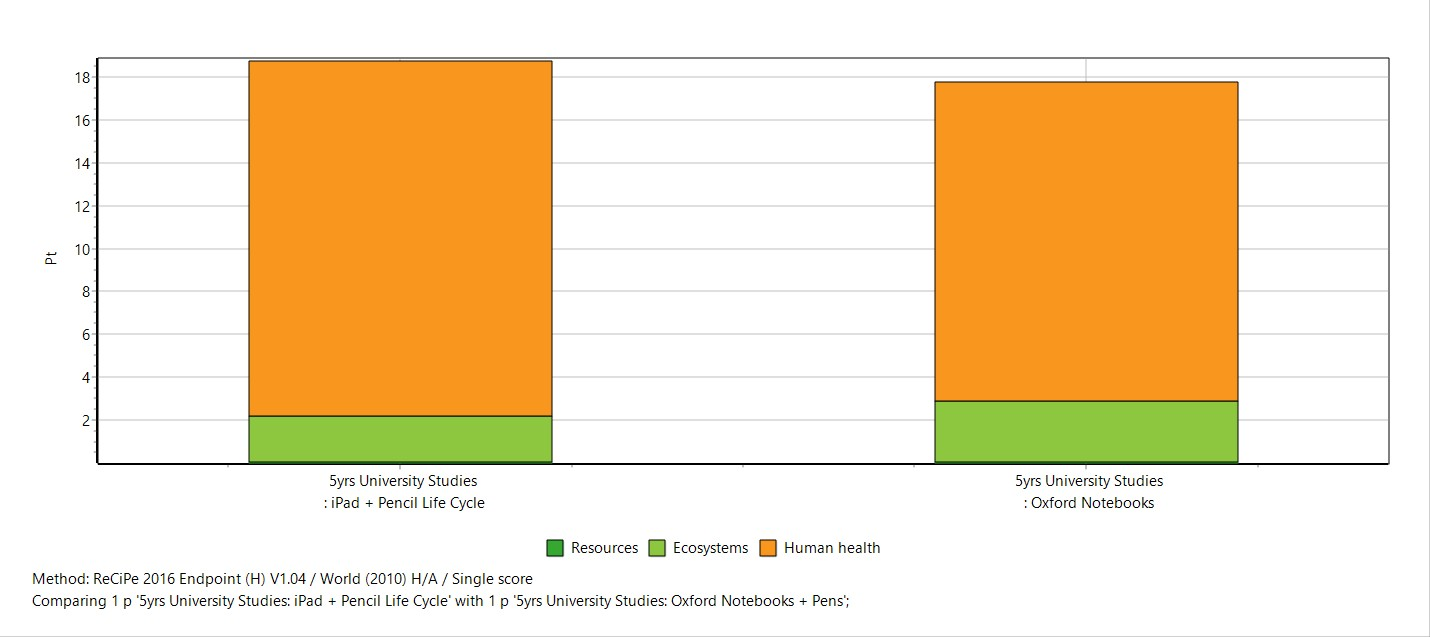
\includegraphics[width=\textwidth]{images/RES_0/Single_Score_RES_0.JPG}
    \caption{caption}\label{fig:single_score_RES0}
\end{figure}

\subsubsection{50\% RES Penetration}

\begin{figure}[H]
    \centering
    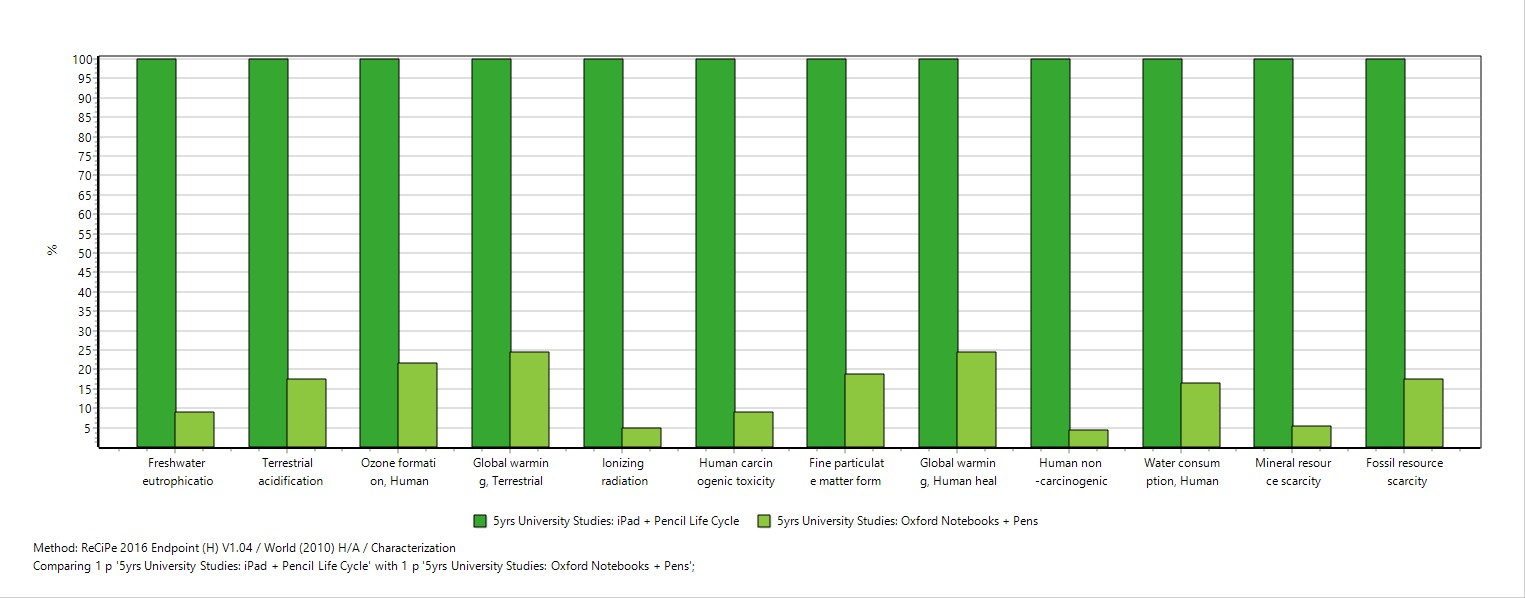
\includegraphics[width=\textwidth]{images/RES_50/Characterization_RES_50.JPG}
    \caption{Relative characterization for a 50\% RES penetration scenario of the investigated note-taking approaches per impact category.}\label{fig:characterization_RES_50}
\end{figure}

\begin{figure}[H]
    \centering
    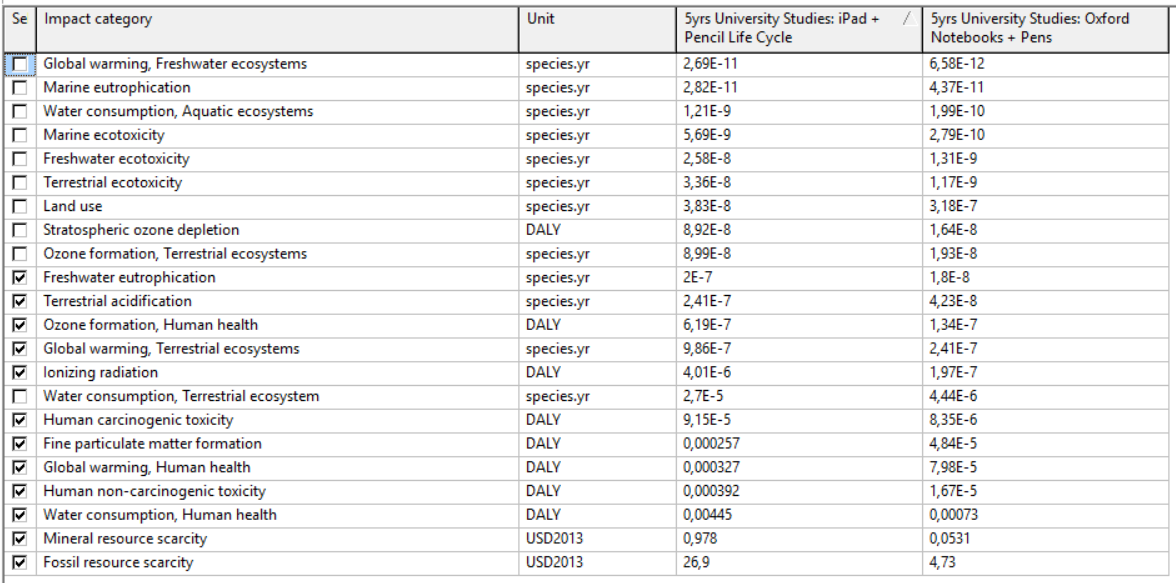
\includegraphics[width=0.9\textwidth]{images/RES_50/Characterization_Table_RES_50.PNG}
    \caption{Absolute characterization for a 50\% RES penetration scenario of the investigated note-taking approaches per impact category.}\label{fig:characterization_table_RES_50}
\end{figure}

\begin{figure}[H]
    \centering
    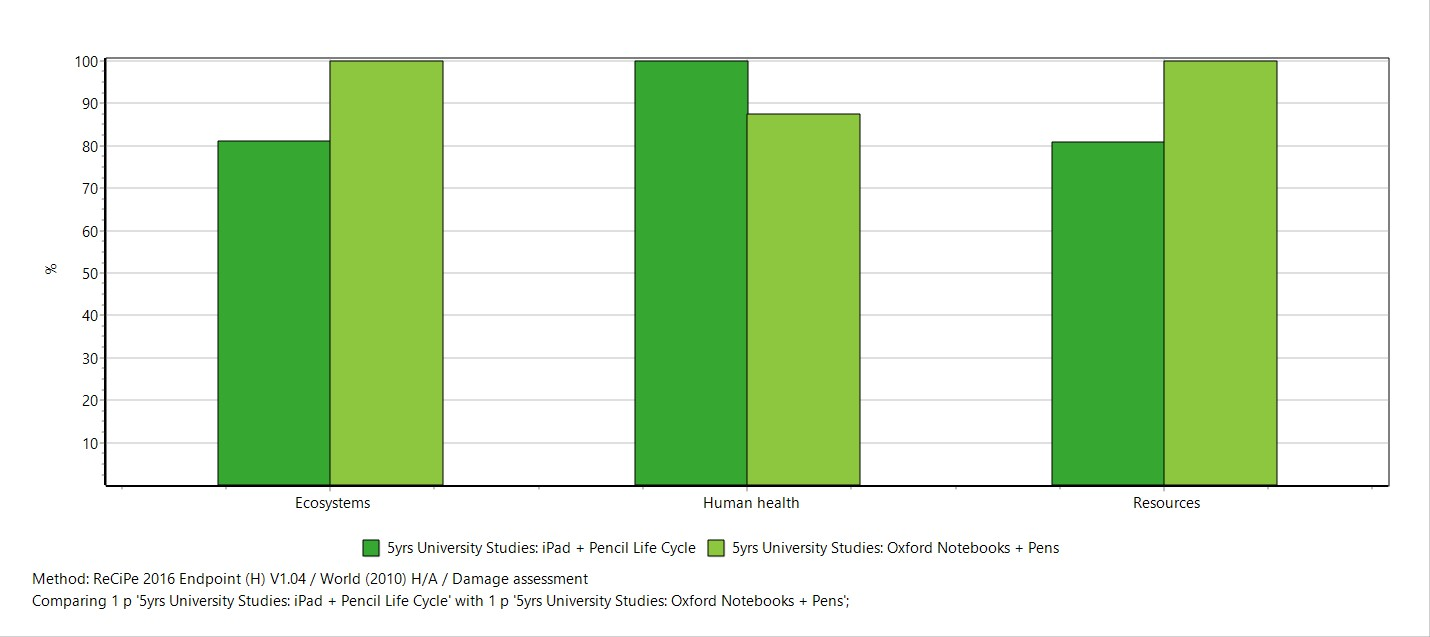
\includegraphics[width=\textwidth]{images/RES_50/Damage_Assessment_RES_50.JPG}
    \caption{caption}\label{fig:damage_assessment_RES_50}
\end{figure}

\begin{figure}[H]
    \centering
    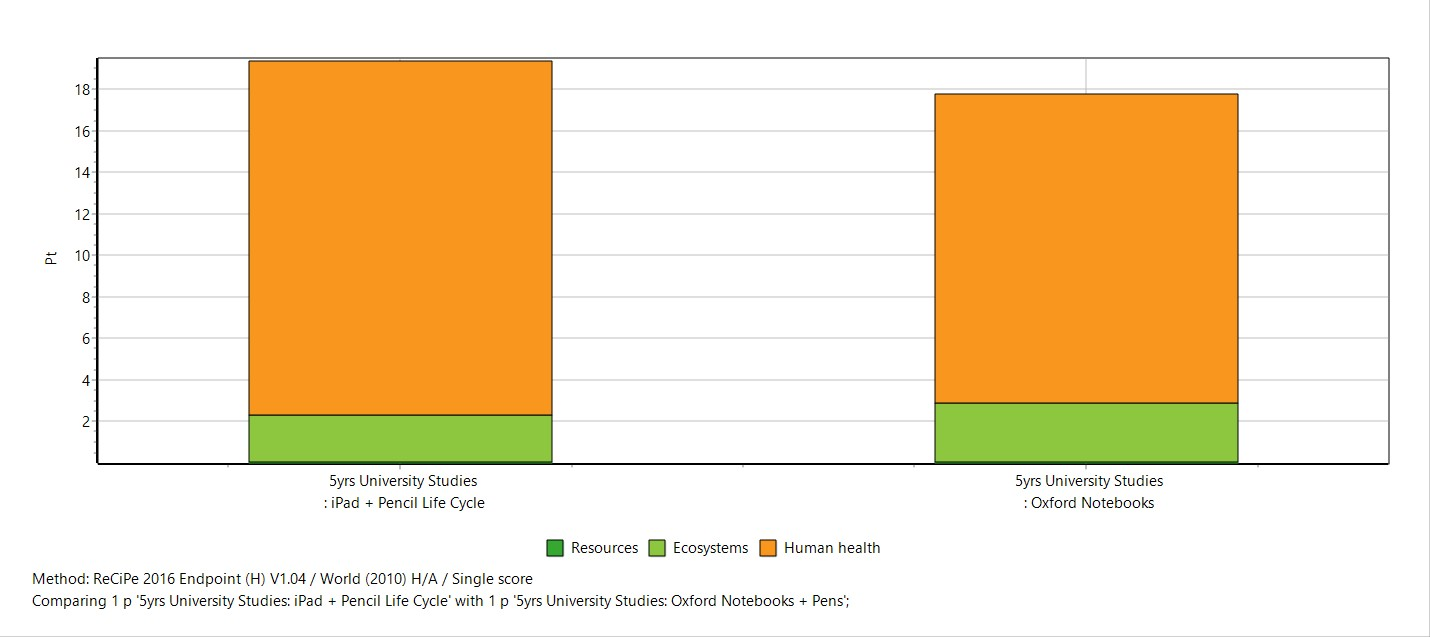
\includegraphics[width=\textwidth]{images/RES_50/Single_Score_RES_50.JPG}
    \caption{caption}\label{fig:single_score_RES50}
\end{figure}

Comparing these findings to the relatively even results from the manufacturing comparison, it can be concluded that the main driving factor for the digital case's impact is its energy source. For this reason, scenarios with increasing RES shares are investigated in the following.

\subsubsection{100\% RES Penetration}

\begin{figure}[H]
    \centering
    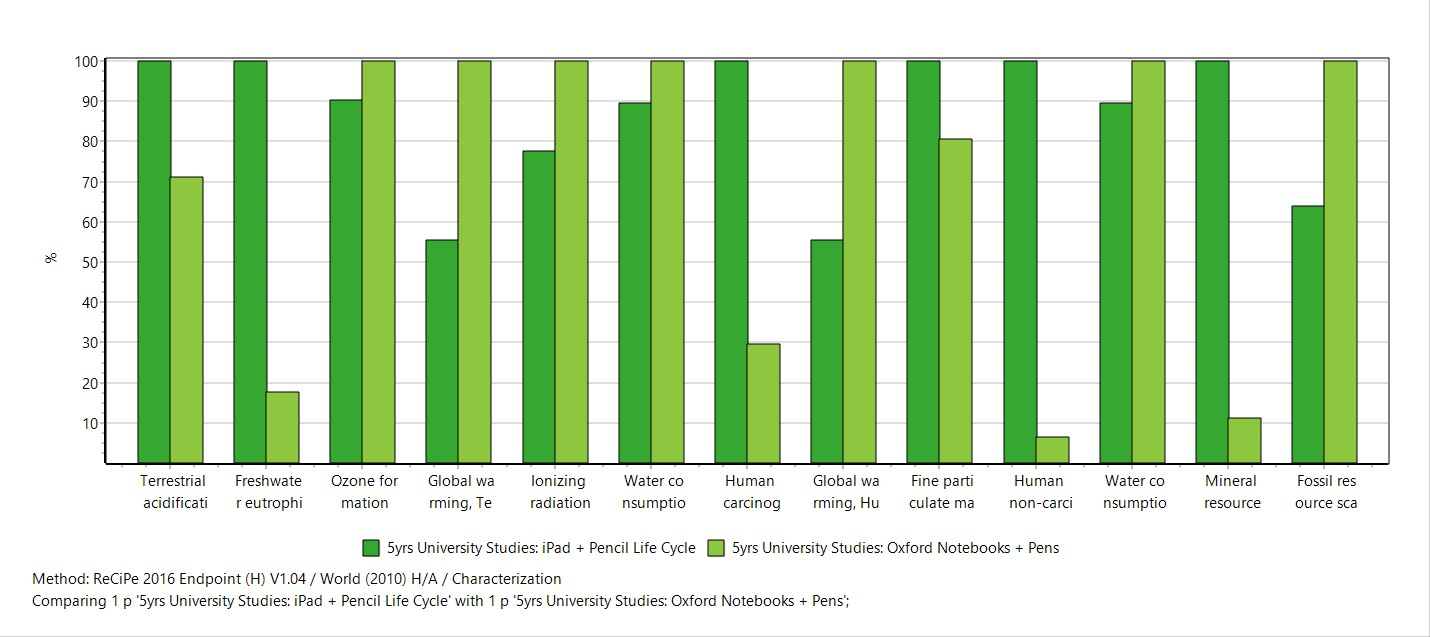
\includegraphics[width=\textwidth]{images/RES_100/Characterization_RES_100.JPG}
    \caption{Relative characterization for a 100\% RES penetration scenario of the investigated note-taking approaches per impact category.}\label{fig:characterization_RES_100}
\end{figure}

\begin{figure}[H]
    \centering
    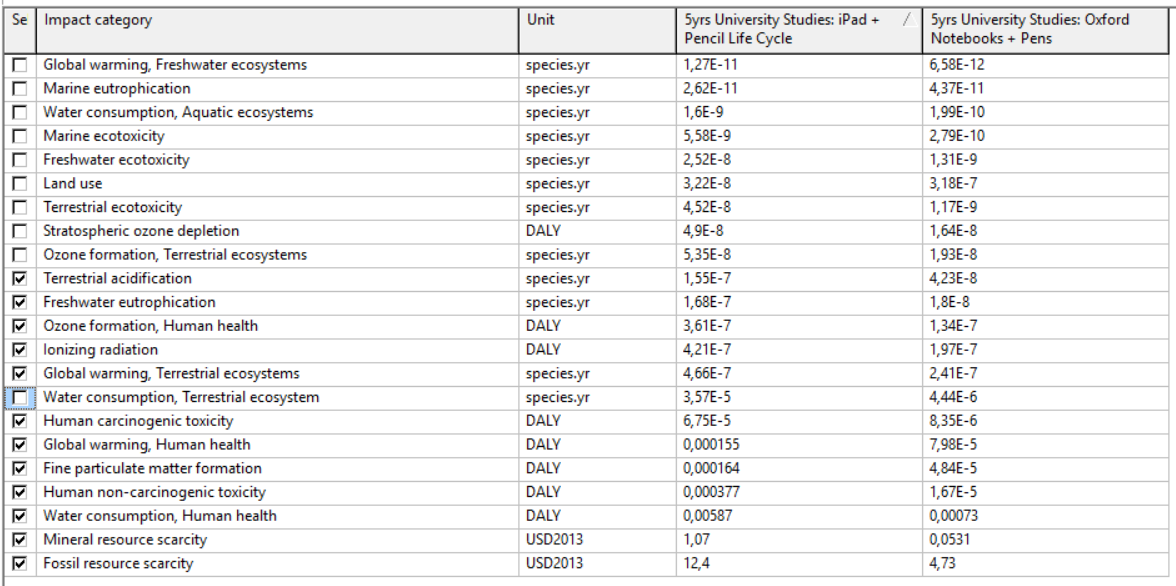
\includegraphics[width=0.9\textwidth]{images/RES_100/Characterization_Table_RES_100.PNG}
    \caption{Absolute characterization for a 100\% RES penetration scenario of the investigated note-taking approaches per impact category.}\label{fig:characterization_table_RES_100}
\end{figure}

\begin{figure}[H]
    \centering
    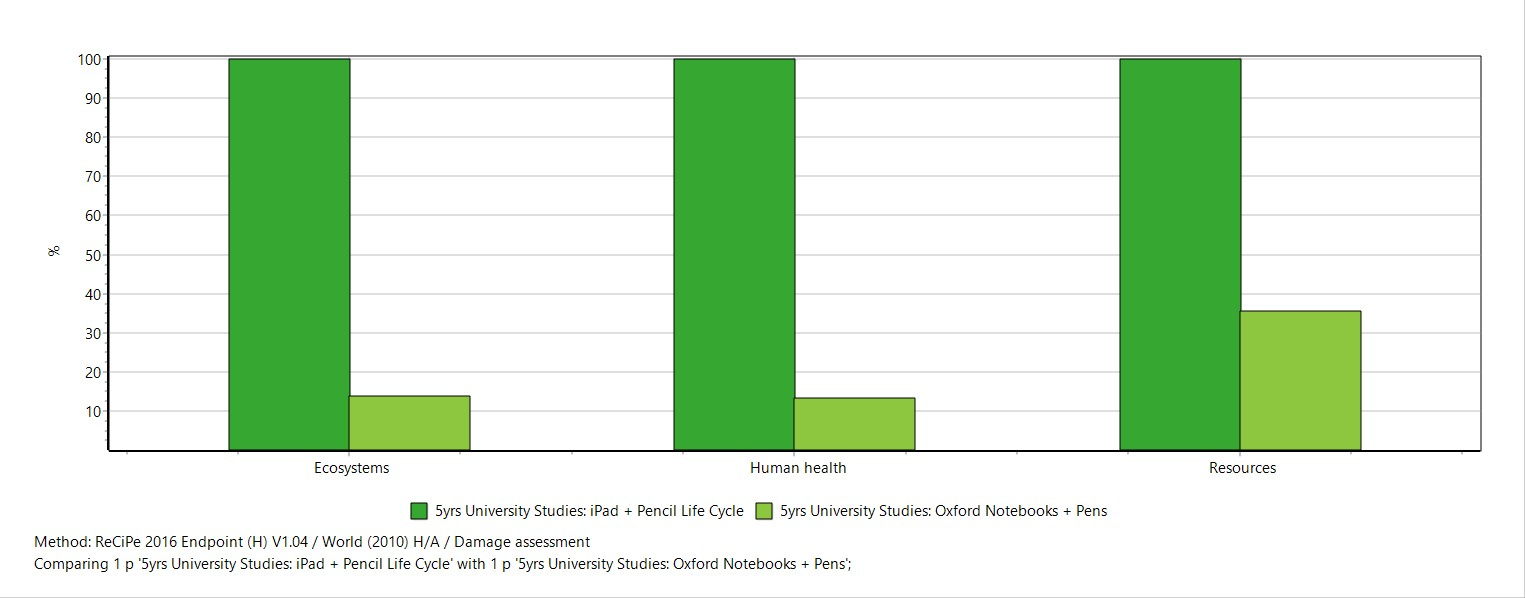
\includegraphics[width=\textwidth]{images/RES_100/Damage_Assessment_RES_100.JPG}
    \caption{caption}\label{fig:damage_assessment_RES_100}
\end{figure}

\begin{figure}[H]
    \centering
    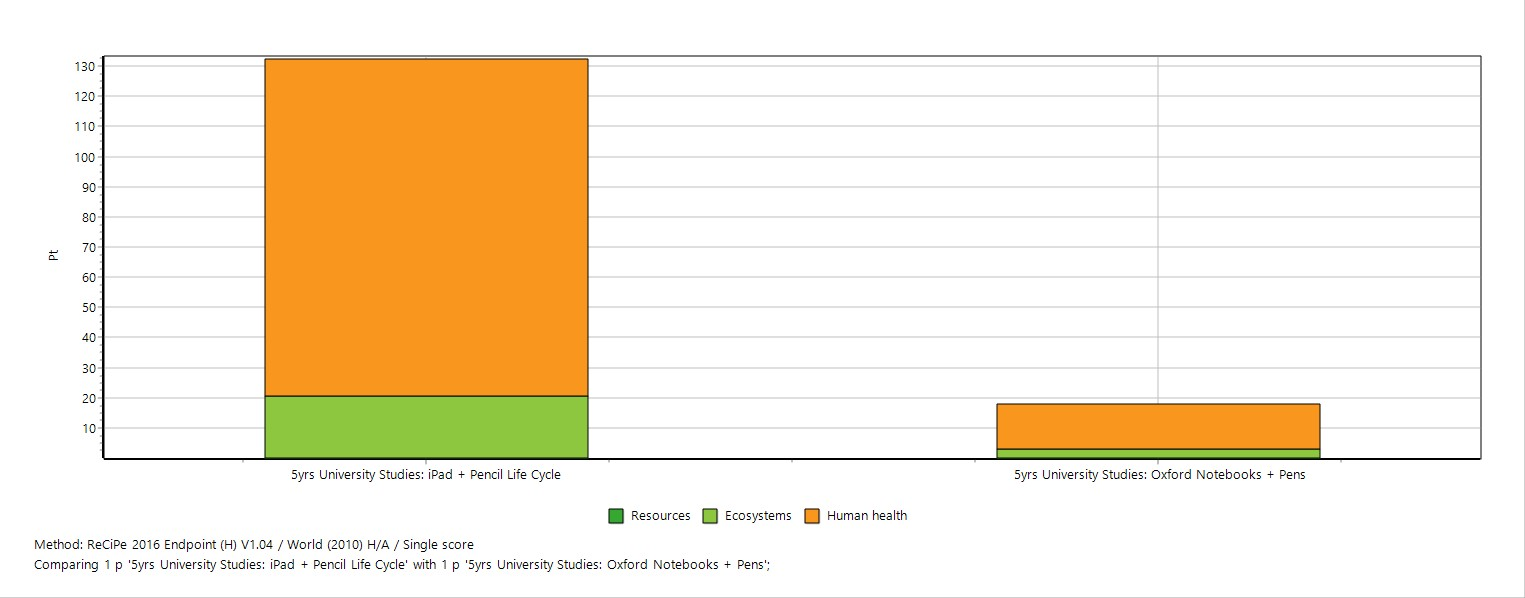
\includegraphics[width=\textwidth]{images/RES_100/Single_Score_RES_100.JPG}
    \caption{caption}\label{fig:single_score_RES100}
\end{figure}